\documentclass[svgnames,11pt]{beamer}
\input{/home/tof/Documents/Cozy/latex-include/preambule_commun.tex}
\input{/home/tof/Documents/Cozy/latex-include/preambule_beamer.tex}
%\usepackage{pgfpages} \setbeameroption{show notes on second screen=left}
\author[]{Christophe Viroulaud}
\title{Recherche dichotomique}
\date{\framebox{\textbf{Algo 03}}}
%\logo{}
\institute{Première - NSI}

\begin{document}
\begin{frame}
\titlepage
\end{frame}

\begin{frame}
    Rechercher un élément dans un tableau est une opération courante. Cette tâche a un coût qui dépend de la taille du tableau.
   

    \begin{center}
        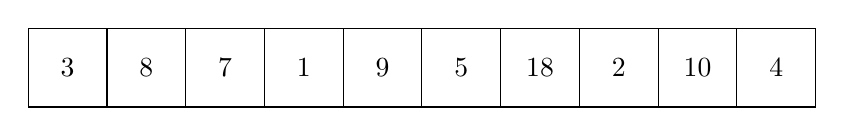
\begin{tikzpicture}
            \draw (0,0) grid (10,1);
            \foreach \x/\n in {0/3,1/8,2/7,3/1,4/9,5/5,6/18,7/2,8/10,9/4}{
                    \node at(0.5+\x,0.5) {\n};
                }
        \end{tikzpicture}
    \end{center}
\begin{itemize}
    \item recherche de 3,
    \item recherche de 9,
    \item recherche de 6.
\end{itemize}
\end{frame}
\begin{frame}
    \frametitle{}
    Cependant, si le tableau est déjà trié est-il possible d'accélérer la recherche?
    \begin{center}
        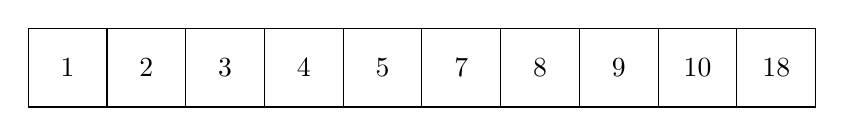
\begin{tikzpicture}
            \draw (0,0) grid (10,1);
            \foreach \x/\n in {0/1,1/2,2/3,3/4,4/5,5/7,6/8,7/9,8/10,9/18}{
                    \node at(0.5+\x,0.5) {\n};
                }
        \end{tikzpicture}
    \end{center}
    \begin{framed}
        \centering Comment implémenter une recherche efficace dans un tableau trié?
   \end{framed}

\end{frame}
\section{Recherche classique dans un tableau}
\subsection{Recherche classique - Génération des données}
\begin{frame}
    \frametitle{Génération des données}
    Imaginons un supermarché qui référence chaque article par un entier. Les références, au nombre de cent mille, sont contenues dans un tableau.

\begin{center}
    \begin{tabular}{*{4}{c}}
        
\includegraphics[width=2cm]{ressources/pomme.jpg}&
        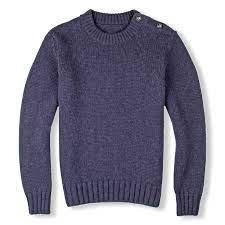
\includegraphics[width=2cm]{ressources/pull.jpg}&
        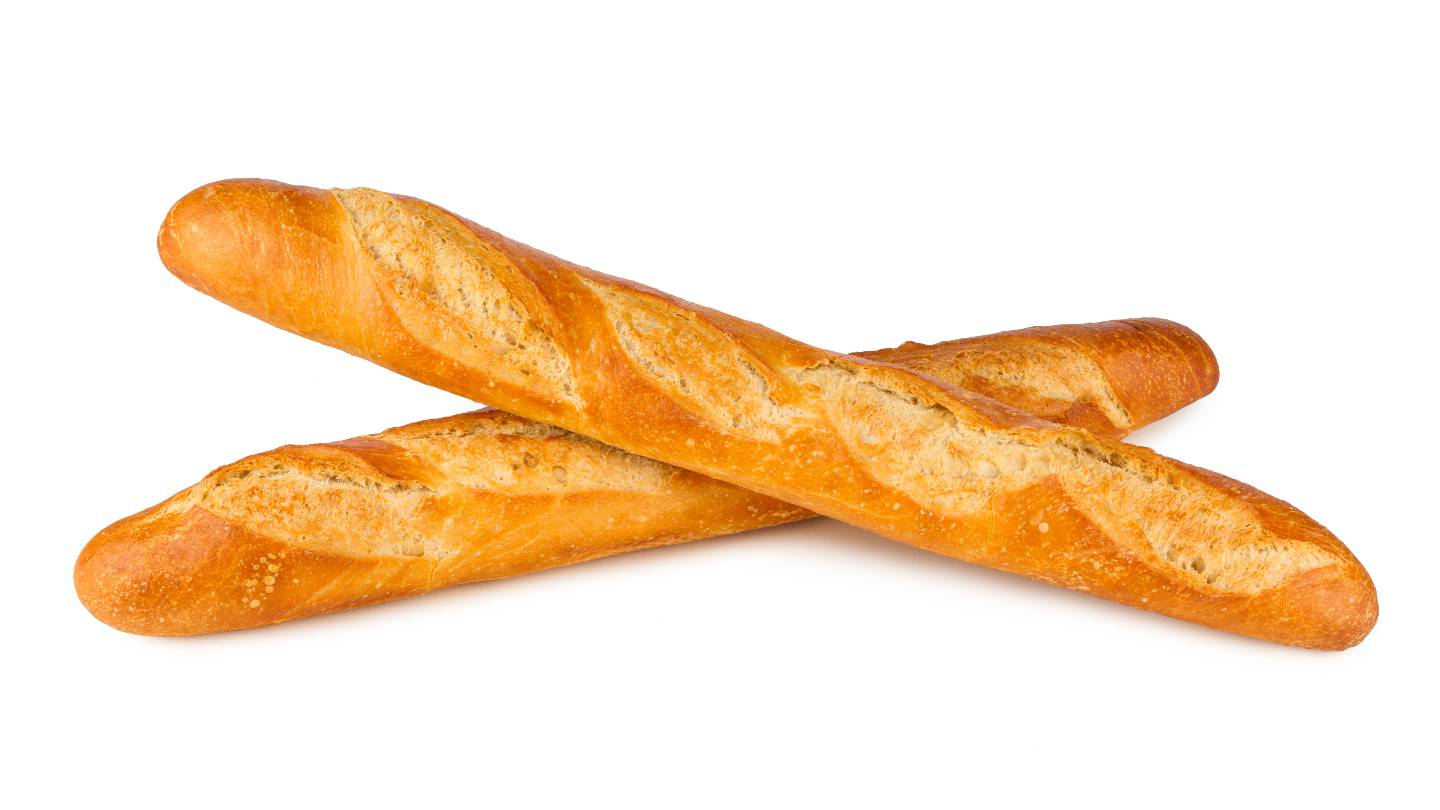
\includegraphics[width=2cm]{ressources/pain.jpg}&
        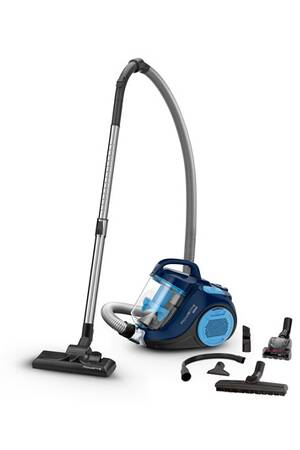
\includegraphics[width=2cm]{ressources/aspirateur.jpg}\\
        12&6780&376&134900\\
    \end{tabular}
\end{center}
\end{frame}
\begin{frame}
    \frametitle{}

    \begin{activite}
        Construire par compréhension un tableau de cent mille entiers compris entre 0 et 1000000.
    \end{activite}

\end{frame}
\begin{frame}[fragile]
    \frametitle{Correction}

    \begin{center}
    \begin{lstlisting}[language=Python , basicstyle=\ttfamily\small, xleftmargin=0.2em, xrightmargin=-1em]
from random import randint

entiers = [randint(0, 1000000) for _ in range(100000)]
\end{lstlisting}
    \captionof*{code}{Jeu de données}
    \label{CODE}
    \end{center}

\end{frame}
\subsection{Recherche dans les données}
\begin{frame}
    \frametitle{Recherche dans les données}

    Pour vérifier la présence d'une valeur dans les données, il faut parcourir le tableau élément par élément.
\begin{center}
    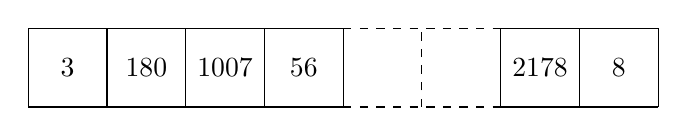
\begin{tikzpicture}
        \draw (0,0)grid(4,1);
        \draw[dashed] (4,0)grid(6,1);
        \draw (6,0)grid(8,1);
        \node at(0.5,0.5){3};
        \node at(1.5,0.5){180};
        \node at(2.5,0.5){1007};
        \node at(3.5,0.5){56};
        \node at(6.5,0.5){2178};
        \node at(7.5,0.5){8};


    \end{tikzpicture}
    \captionof{figure}{Parcours séquentiel}
\end{center}

\end{frame}
\begin{frame}
    \frametitle{Dans le pire des cas}

    \begin{center}
        \begin{tabular}{|c|c|}
            \hline
            nombre d'éléments&nombre de comparaisons\\
            \hline
            100&100\\
            10000&10000\\
            1000000&1000000\\
            \hline
        \end{tabular}
    \end{center}

\end{frame}
\begin{frame}
    \frametitle{}

    \begin{aretenir}[]
        Dans le pire des cas le nombre d'opérations de la recherche dépend du nombre d'éléments.\\
        \centering La complexité est \textbf{linéaire}.
        \end{aretenir}
\note{cas où l'élément n'est pas présent}
\end{frame}

\begin{frame}[fragile]
    \frametitle{}

    \begin{activite}
        \begin{enumerate}
            \item Écrire la fonction \textbf{\texttt{recherche\_classique(tab: list, cherche: int) $\rightarrow$ bool}} qui renvoie \textbf{\texttt{True}} si l'entier \textbf{\texttt{cherche}} est présent dans le tableau.
            \item Tester la fonction: vérifier si le nombre 575000 a été choisi par une personne.
        \end{enumerate}
    \end{activite} 
\end{frame}
\begin{frame}[fragile]
    \frametitle{Correction}

    \begin{center}
        \lstinputlisting[firstline=12 ,lastline=21, basicstyle=\ttfamily\small , xleftmargin=0.2em, xrightmargin=-2.5em]{"scripts/dicho.py"}
        \captionof{code}{Création de la fonction}
    \end{center}

    \begin{center}
    \begin{lstlisting}[language=Python , basicstyle=\ttfamily\small, xleftmargin=0.2em, xrightmargin=-2em]
entiers = [randint(0, 1000000) for _ in range(100000)]
recherche_classique(entiers, 57500)
\end{lstlisting}
    \captionof{code}{Utilisation de la fonction}
    \label{CODE}
    \end{center}
\end{frame}
\begin{frame}[fragile]
    \frametitle{}
    \setcounter{compteuractivite}{1}

    \begin{activite}
        Dans le programme principal, créer une variable \textbf{\texttt{COMPTEUR}} initialisée à 0. Cette variable de test sera utilisée \emph{dans la fonction} pour compter le nombre d'itérations de la boucle de recherche. On parle alors de \textbf{variable globale} car elle n'est pas propre à la fonction. Il faudra ajouter le code \ref{global} au début de la fonction.
        \begin{center}
        \begin{lstlisting}[language=Python  , xleftmargin=2em, xrightmargin=2em]
global COMPTEUR
\end{lstlisting}
        \captionof{code}{Déclaration d'une variable globale}
        \label{global}
        \end{center}
    \end{activite}

\end{frame}
\begin{frame}[fragile]
    \frametitle{Correction}

\begin{center}
\begin{lstlisting}[language=Python , basicstyle=\ttfamily\small, xleftmargin=0.2em, xrightmargin=-2.5em]
COMPTEUR = 0

def recherche_classique(tab: list, cherche: int) -> bool:
    """
    Renvoie True si 'cherche' est dans 'tab'
    """
    global COMPTEUR
    for element in tab:
        COMPTEUR += 1
        if element == cherche:
            return True
    # à la fin de la boucle on n'a pas trouvé 'cherche'
    return False
\end{lstlisting}
\end{center}
\begin{center}
    \begin{lstlisting}[language=Python , basicstyle=\ttfamily\small, xleftmargin=2em, xrightmargin=2em]
print(recherche_classique(entiers, 57500))
print(COMPTEUR)
\end{lstlisting}
    \captionof{code}{Utilisation de la fonction}
    \label{CODE}
    \end{center}
\end{frame}
\begin{frame}
    \frametitle{}

    \begin{aretenir}[]
    La variable \textbf{\texttt{COMPTEUR}} est utilisée ici uniquement pour effectuer des tests. \\\textbf{D'une manière générale, \underline{modifier} une variable globale dans une fonction est une mauvaise pratique.}
    \end{aretenir}

\end{frame}
\section{Recherche dans un tableau trié}
\subsection{Dans un tableau trié - Des données ordonnées}
\begin{frame}
    \frametitle{Des données ordonnées}
    Considérons maintenant que les références sont triées par ordre croissant au fur et à mesure de leur ajout dans le tableau de données.
\begin{center}
    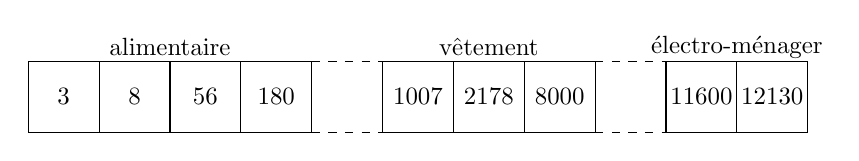
\begin{tikzpicture}[scale=0.9, transform shape]
        \draw (0,0)grid(4,1);
        \draw[dashed] (4,0)grid(5,1);
        \draw (5,0)grid(8,1);
        \draw[dashed] (8,0)grid(9,1);
        \draw (9,0)grid(11,1);
        \node at(0.5,0.5){3};
        \node at(1.5,0.5){8};
        \node at(2.5,0.5){56};
        \node at(3.5,0.5){180};
        \node at(5.5,0.5){1007};
        \node at(6.5,0.5){2178};
        \node at(7.5,0.5){8000};
        \node at(9.5,0.5){11600};
        \node at(10.5,0.5){12130};
        \node at(2,1.2){alimentaire};
        \node at(6.5,1.2){vêtement};
        \node at(10,1.2){électro-ménager};

    \end{tikzpicture}
    \captionof{figure}{Références triées}
\end{center}

\end{frame}
\begin{frame}
    \frametitle{}

    \begin{activite}
        Pour simplifier nous allons utiliser la méthode \textbf{\texttt{sort}} pour trier les données.
        \begin{enumerate}
            \item Construire par compréhension un tableau de cent mille entiers compris entre 0 et 1000000.
            \item Trier le tableau.
        \end{enumerate}
        \end{activite}

\end{frame}
\begin{frame}[fragile]
    \frametitle{Correction}

    \begin{center}
    \begin{lstlisting}[language=Python , basicstyle=\ttfamily\small, xleftmargin=0.2em, xrightmargin=-1.8em]
entiers = [randint(0, 1000000) for _ in range(100000)]
entiers.sort()
\end{lstlisting}
    \captionof*{code}{Jeu de données}
    \label{CODE}
    \end{center}

\end{frame}
\subsection{Recherche dichotomique}
\begin{frame}
    \frametitle{Recherche dichotomique}

    Les données étant triées, le principe de la dichotomie, pour chercher la présence d'un élément, consiste à:
\begin{itemize}
    \item couper le tableau en deux parties égales,
    \item ne garder que la partie contenant l'élément,
    \item répéter l'opération jusqu'à trouver l'élément ou bien avoir une partie vide.
\end{itemize}
\note{à peu près égales selon parité}
\end{frame}
\begin{frame}
    \frametitle{}

    Cherchons 302 dans le tableau suivant:
\begin{center}
    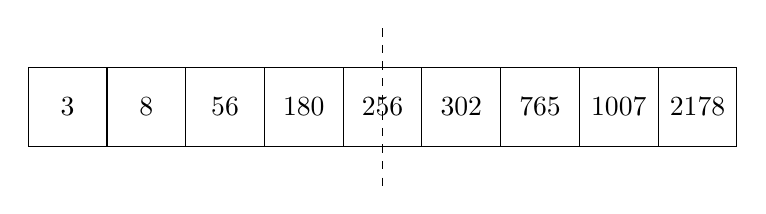
\begin{tikzpicture}
        \draw (0,0)grid(9,1);
        \node at(0.5,0.5){3};
        \node at(1.5,0.5){8};
        \node at(2.5,0.5){56};
        \node at(3.5,0.5){180};
        \node at(4.5,0.5){256};
        \node at(5.5,0.5){302};
        \node at(6.5,0.5){765};
        \node at(7.5,0.5){1007};
        \node at(8.5,0.5){2178};
        \draw[dashed] (4.5,1.5)--(4.5,-0.5);
    \end{tikzpicture}
    \captionof{figure}{Séparons les données en deux parties}
\end{center}

\end{frame}
\begin{frame}
    \frametitle{}

    \begin{center}
        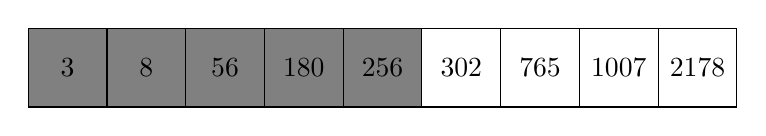
\begin{tikzpicture}
            \fill[gray] (0,0) -- (5,0) -- (5,1) -- (0,1)-- cycle;
            \draw (0,0)grid(9,1);
            \node at(0.5,0.5){3};
            \node at(1.5,0.5){8};
            \node at(2.5,0.5){56};
            \node at(3.5,0.5){180};
            \node at(4.5,0.5){256};
            \node at(5.5,0.5){302};
            \node at(6.5,0.5){765};
            \node at(7.5,0.5){1007};
            \node at(8.5,0.5){2178};
        \end{tikzpicture}
        \captionof{figure}{256 n'est pas le nombre recherché et il est inférieur à 302}
    \end{center} 

\end{frame}
\begin{frame}
    \frametitle{}

    \begin{center}
        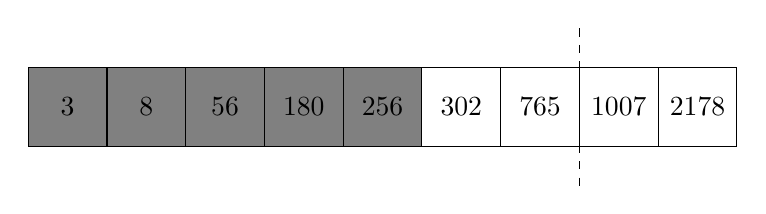
\begin{tikzpicture}
            \fill[gray] (0,0) -- (5,0) -- (5,1) -- (0,1)-- cycle;
            \draw (0,0)grid(9,1);
            \node at(0.5,0.5){3};
            \node at(1.5,0.5){8};
            \node at(2.5,0.5){56};
            \node at(3.5,0.5){180};
            \node at(4.5,0.5){256};
            \node at(5.5,0.5){302};
            \node at(6.5,0.5){765};
            \node at(7.5,0.5){1007};
            \node at(8.5,0.5){2178};
            \draw[dashed] (7,1.5)--(7,-0.5);
        \end{tikzpicture}
        \captionof{figure}{Séparons les données restantes en deux parties}
    \end{center}

\end{frame}
\begin{frame}
    \frametitle{}

    \begin{center}
        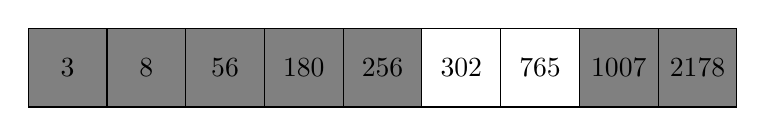
\begin{tikzpicture}
            \fill[gray] (0,0) -- (5,0) -- (5,1) -- (0,1)-- cycle;
            \fill[gray] (7,0) -- (9,0) -- (9,1) -- (7,1)-- cycle;
            \draw (0,0)grid(9,1);
            \node at(0.5,0.5){3};
            \node at(1.5,0.5){8};
            \node at(2.5,0.5){56};
            \node at(3.5,0.5){180};
            \node at(4.5,0.5){256};
            \node at(5.5,0.5){302};
            \node at(6.5,0.5){765};
            \node at(7.5,0.5){1007};
            \node at(8.5,0.5){2178};
        \end{tikzpicture}
        \captionof{figure}{Nous pouvons éliminer la partie supérieure.}
    \end{center}

\end{frame}
\begin{frame}
    \frametitle{}

    \begin{center}
        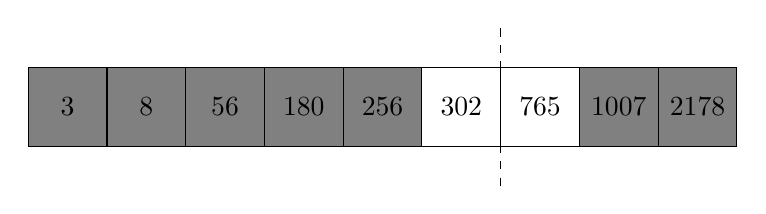
\begin{tikzpicture}
            \fill[gray] (0,0) -- (5,0) -- (5,1) -- (0,1)-- cycle;
            \fill[gray] (7,0) -- (9,0) -- (9,1) -- (7,1)-- cycle;
            \draw (0,0)grid(9,1);
            \node at(0.5,0.5){3};
            \node at(1.5,0.5){8};
            \node at(2.5,0.5){56};
            \node at(3.5,0.5){180};
            \node at(4.5,0.5){256};
            \node at(5.5,0.5){302};
            \node at(6.5,0.5){765};
            \node at(7.5,0.5){1007};
            \node at(8.5,0.5){2178};
            \draw[dashed] (6,1.5)--(6,-0.5);
        \end{tikzpicture}
        \captionof{figure}{Dernière séparation}
    \end{center}

\end{frame}
\begin{frame}
    \frametitle{}

    \begin{center}
        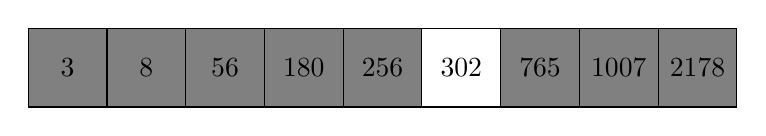
\begin{tikzpicture}
            \fill[gray] (0,0) -- (5,0) -- (5,1) -- (0,1)-- cycle;
            \fill[gray] (6,0) -- (9,0) -- (9,1) -- (6,1)-- cycle;
            \draw (0,0)grid(9,1);
            \node at(0.5,0.5){3};
            \node at(1.5,0.5){8};
            \node at(2.5,0.5){56};
            \node at(3.5,0.5){180};
            \node at(4.5,0.5){256};
            \node at(5.5,0.5){302};
            \node at(6.5,0.5){765};
            \node at(7.5,0.5){1007};
            \node at(8.5,0.5){2178};
        \end{tikzpicture}
        \captionof{figure}{302 a été trouvée en trois itérations}
    \end{center}

\end{frame}
\begin{frame}[fragile]
    \frametitle{}
    \begin{aretenir}[Remarque]
        En pratique, on utilise les indices pour trouver le milieu.
    \end{aretenir}
    \begin{center}
        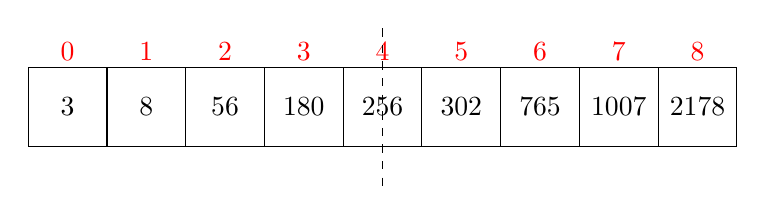
\begin{tikzpicture}
            \draw (0,0)grid(9,1);
            \foreach \a/\b in {0/3, 1/8, 2/56, 3/180, 4/256, 5/302, 6/765, 7/1007, 8/2178}
            {\node at (\a+0.5,0.5) {\b};
            \node[red] at (\a+0.5,1.2) {\a};}
            \draw[dashed] (4.5,1.5)--(4.5,-0.5);
        \end{tikzpicture}
        \captionof{figure}{$\dfrac{8+0}{2}=4$ l'indice médian est 4}
    \end{center}
\begin{center}
\begin{lstlisting}[language=Python , basicstyle=\ttfamily\small, xleftmargin=2em, xrightmargin=2em]
i_debut = 0
i_fin = 8
\end{lstlisting}
\end{center}
\end{frame}
\begin{frame}
    

    \begin{center}
        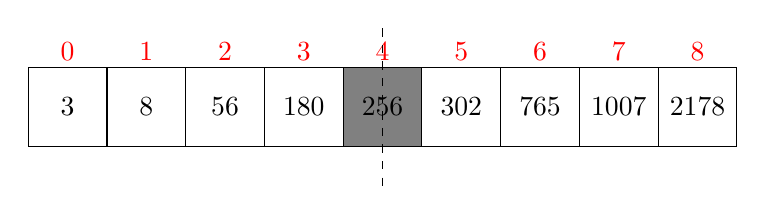
\begin{tikzpicture}
            \fill[gray] (4,0) -- (5,0) -- (5,1) -- (4,1)-- cycle;
            \draw (0,0)grid(9,1);
            \foreach \a/\b in {0/3, 1/8, 2/56, 3/180, 4/256, 5/302, 6/765, 7/1007, 8/2178}
            {\node at (\a+0.5,0.5) {\b};
            \node[red] at (\a+0.5,1.2) {\a};}
            \draw[dashed] (4.5,1.5)--(4.5,-0.5);
        \end{tikzpicture}
        \captionof{figure}{256 n'est pas le nombre recherché}
    \end{center}
\end{frame}
\begin{frame}[fragile]

    \begin{center}
        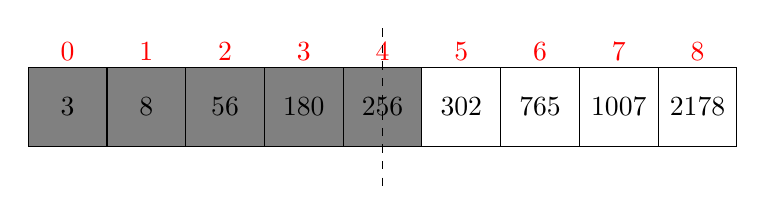
\begin{tikzpicture}
            \fill[gray] (0,0) -- (5,0) -- (5,1) -- (0,1)-- cycle;
            \draw (0,0)grid(9,1);
            \foreach \a/\b in {0/3, 1/8, 2/56, 3/180, 4/256, 5/302, 6/765, 7/1007, 8/2178}
            {\node at (\a+0.5,0.5) {\b};
            \node[red] at (\a+0.5,1.2) {\a};}
            \draw[dashed] (4.5,1.5)--(4.5,-0.5);
        \end{tikzpicture}
        \captionof{figure}{256 est inférieur au nombre recherché.}
    \end{center}
    \begin{center}
\begin{lstlisting}[language=Python , basicstyle=\ttfamily\small, xleftmargin=2em, xrightmargin=2em]
i_debut = 5
i_fin = 8
\end{lstlisting}
        \end{center}
\end{frame}

\begin{frame}
    \frametitle{}

    \begin{center}
        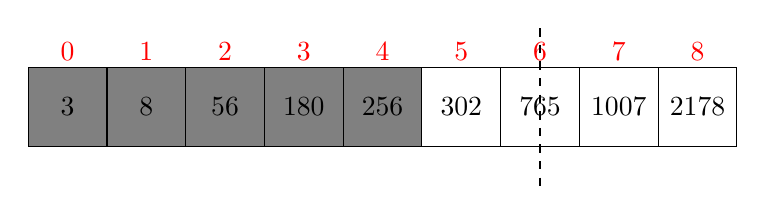
\begin{tikzpicture}
            \fill[gray] (0,0) -- (5,0) -- (5,1) -- (0,1)-- cycle;
            \draw (0,0)grid(9,1);
            \foreach \a/\b in {0/3, 1/8, 2/56, 3/180, 4/256, 5/302, 6/765, 7/1007, 8/2178}
            {\node at (\a+0.5,0.5) {\b};
            \node[red] at (\a+0.5,1.2) {\a};}
            \draw[dashed] (6.5,1.5)--(6.5,-0.5);
        \end{tikzpicture}
        \captionof{figure}{$\dfrac{8+5}{2}=6$ l'indice médian est 6}
    \end{center}
\note[item]{l'indice est un entier}
\end{frame}
\begin{frame}
    \frametitle{}

    \begin{center}
        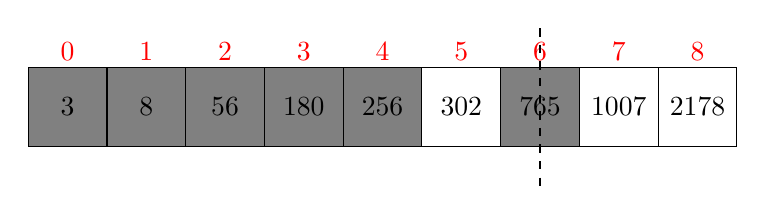
\begin{tikzpicture}
            \fill[gray] (0,0) -- (5,0) -- (5,1) -- (0,1)-- cycle;
            \fill[gray] (6,0) -- (7,0) -- (7,1) -- (6,1)-- cycle;
            \draw (0,0)grid(9,1);
            \foreach \a/\b in {0/3, 1/8, 2/56, 3/180, 4/256, 5/302, 6/765, 7/1007, 8/2178}
            {\node at (\a+0.5,0.5) {\b};
            \node[red] at (\a+0.5,1.2) {\a};}
            \draw[dashed] (6.5,1.5)--(6.5,-0.5);
        \end{tikzpicture}
        \captionof{figure}{765 n'est pas le nombre recherché.}
    \end{center}
\note[item]{l'indice est un entier}
\end{frame}
\begin{frame}[fragile]
    \frametitle{}

    \begin{center}
        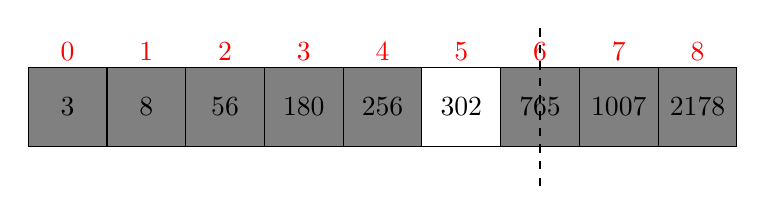
\begin{tikzpicture}
            \fill[gray] (0,0) -- (5,0) -- (5,1) -- (0,1)-- cycle;
            \fill[gray] (6,0) -- (9,0) -- (9,1) -- (6,1)-- cycle;
            \draw (0,0)grid(9,1);
            \foreach \a/\b in {0/3, 1/8, 2/56, 3/180, 4/256, 5/302, 6/765, 7/1007, 8/2178}
            {\node at (\a+0.5,0.5) {\b};
            \node[red] at (\a+0.5,1.2) {\a};}
            \draw[dashed] (6.5,1.5)--(6.5,-0.5);
        \end{tikzpicture}
        \captionof{figure}{765 est supérieur au nombre recherché.}
    \end{center}
    \begin{center}
        \begin{lstlisting}[language=Python , basicstyle=\ttfamily\small, xleftmargin=2em, xrightmargin=2em]
i_debut = 5
i_fin = 5
\end{lstlisting}
                \end{center}
\end{frame}
\begin{frame}
    \frametitle{}

    \begin{center}
        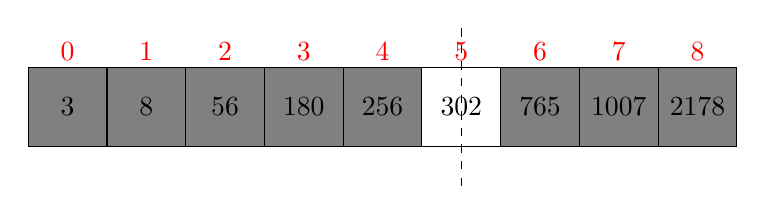
\begin{tikzpicture}
            \fill[gray] (0,0) -- (5,0) -- (5,1) -- (0,1)-- cycle;
            \fill[gray] (6,0) -- (9,0) -- (9,1) -- (6,1)-- cycle;
            \draw (0,0)grid(9,1);
            \foreach \a/\b in {0/3, 1/8, 2/56, 3/180, 4/256, 5/302, 6/765, 7/1007, 8/2178}
            {\node at (\a+0.5,0.5) {\b};
            \node[red] at (\a+0.5,1.2) {\a};}
            \draw[dashed] (5.5,1.5)--(5.5,-0.5);
        \end{tikzpicture}
        \captionof{figure}{$\dfrac{5+5}{2}=5$ l'indice médian est 5.}
    \end{center}
\note{cette dernière itération est nécessaire: on ne sait pas si le dernier élément est bien celui recherché.}
\end{frame}
\begin{frame}
    \frametitle{}

    \begin{center}
        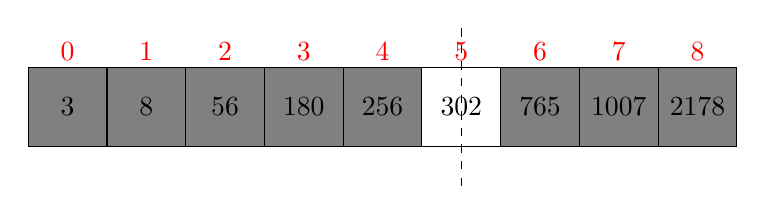
\begin{tikzpicture}
            \fill[gray] (0,0) -- (5,0) -- (5,1) -- (0,1)-- cycle;
            \fill[gray] (6,0) -- (9,0) -- (9,1) -- (6,1)-- cycle;
            \draw (0,0)grid(9,1);
            \foreach \a/\b in {0/3, 1/8, 2/56, 3/180, 4/256, 5/302, 6/765, 7/1007, 8/2178}
            {\node at (\a+0.5,0.5) {\b};
            \node[red] at (\a+0.5,1.2) {\a};}
            \draw[dashed] (5.5,1.5)--(5.5,-0.5);
        \end{tikzpicture}
        \captionof{figure}{On a trouvé l'élément.}
    \end{center}
\end{frame}
\begin{frame}
    \frametitle{}

    
    \begin{activite}
        Écrire la fonction \textbf{\texttt{recherche\_dicho(tab: list, cherche: int) $\rightarrow$ bool}} qui applique le principe de la dichotomie:
        \begin{itemize}
            \item Définir les indices \textbf{\texttt{i\_debut}} et \textbf{\texttt{i\_fin}}.
            \item Tant que \textbf{\texttt{i\_fin $\geq$ i\_debut}}
            \begin{itemize}
                \item Calculer \textbf{\texttt{i\_milieu}}
                \item Vérifier si l'élément d'indice \textbf{\texttt{i\_milieu}} est celui cherché
                \item Sinon redéfinir \textbf{\texttt{i\_debut}} et \textbf{\texttt{i\_fin}} pour ne garder que la partie contenant l'élément cherché.
            \end{itemize} 
        \end{itemize}
        \end{activite}
\end{frame}
\begin{frame}
    \frametitle{Correction}
    \begin{center}
        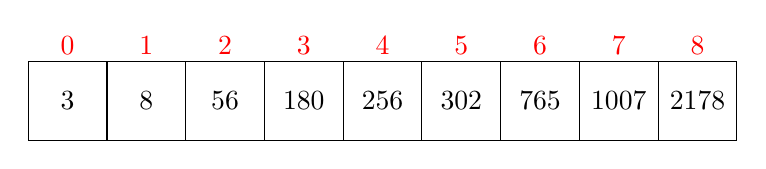
\begin{tikzpicture}
            \draw (0,0)grid(9,1);
            \foreach \a/\b in {0/3, 1/8, 2/56, 3/180, 4/256, 5/302, 6/765, 7/1007, 8/2178}
            {\node at (\a+0.5,0.5) {\b};
            \node[red] at (\a+0.5,1.2) {\a};}
        \end{tikzpicture}
    \end{center}
    \lstinputlisting[firstline=23 ,lastline=25 , basicstyle=\ttfamily\small, xleftmargin=0.2em, xrightmargin=-1.7em]{"scripts/dicho.py"}

\end{frame}
\begin{frame}
    \frametitle{Correction}
    \begin{center}
        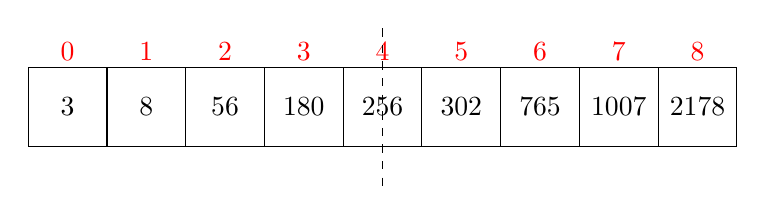
\begin{tikzpicture}
            \draw (0,0)grid(9,1);
            \foreach \a/\b in {0/3, 1/8, 2/56, 3/180, 4/256, 5/302, 6/765, 7/1007, 8/2178}
            {\node at (\a+0.5,0.5) {\b};
            \node[red] at (\a+0.5,1.2) {\a};}
            \draw[dashed] (4.5,1.5)--(4.5,-0.5);
        \end{tikzpicture}
    \end{center}
    \lstinputlisting[firstline=26 ,lastline=27 , basicstyle=\ttfamily\small, xleftmargin=2em, xrightmargin=2em]{"scripts/dicho.py"}
\note{si on ne trouve pas l'élément \textbf{\texttt{i\_fin < i\_debut}}}
\end{frame}
\begin{frame}
    \frametitle{Correction}
    \begin{center}
        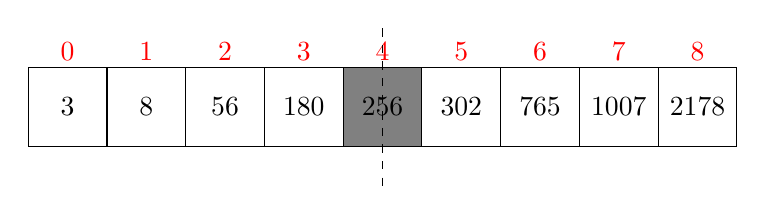
\begin{tikzpicture}
            \fill[gray] (4,0) -- (5,0) -- (5,1) -- (4,1)-- cycle;
            \draw (0,0)grid(9,1);
            \foreach \a/\b in {0/3, 1/8, 2/56, 3/180, 4/256, 5/302, 6/765, 7/1007, 8/2178}
            {\node at (\a+0.5,0.5) {\b};
            \node[red] at (\a+0.5,1.2) {\a};}
            \draw[dashed] (4.5,1.5)--(4.5,-0.5);
        \end{tikzpicture}
    \end{center}
    \lstinputlisting[firstline=28 ,lastline=29 , basicstyle=\ttfamily\small, xleftmargin=2em, xrightmargin=2em]{"scripts/dicho.py"}

\end{frame}
\begin{frame}
    \frametitle{Correction}
    \begin{center}
        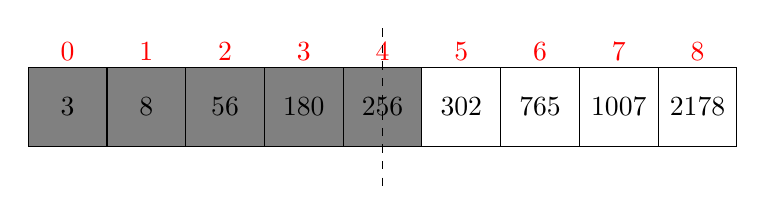
\begin{tikzpicture}
            \fill[gray] (0,0) -- (5,0) -- (5,1) -- (0,1)-- cycle;
            \draw (0,0)grid(9,1);
            \foreach \a/\b in {0/3, 1/8, 2/56, 3/180, 4/256, 5/302, 6/765, 7/1007, 8/2178}
            {\node at (\a+0.5,0.5) {\b};
            \node[red] at (\a+0.5,1.2) {\a};}
            \draw[dashed] (4.5,1.5)--(4.5,-0.5);
        \end{tikzpicture}
    \end{center}
    \lstinputlisting[firstline=30 ,lastline=33 , basicstyle=\ttfamily\small, xleftmargin=2em, xrightmargin=2em]{"scripts/dicho.py"}

\end{frame}
\begin{frame}
    \frametitle{Correction}

    \lstinputlisting[firstline=23 ,lastline=36 , basicstyle=\ttfamily\small, xleftmargin=0.2em, xrightmargin=-1.7em]{"scripts/dicho.py"}

\end{frame}
\subsection{Efficacité}
\begin{frame}
    \frametitle{Efficacité}

    \begin{activite}
        \begin{enumerate}
            \item En utilisant une variable \textbf{\texttt{COMPTEUR}}, compter le nombre d'itérations de la boucle de recherche dichotomique.
            \item Tester pour différentes tailles de tableau.
        \end{enumerate}
        \end{activite}

\end{frame}
\begin{frame}[fragile]
    \frametitle{Correction}

\begin{center}
\begin{lstlisting}[language=Python , basicstyle=\ttfamily\small, xleftmargin=0.2em, xrightmargin=-1.7em]
COMPTEUR = 0

def recherche_dicho(tab: list, cherche: int) -> bool:
    global COMPTEUR
    i_debut = 0
    i_fin = len(tab)-1
    while i_fin >= i_debut:
        COMPTEUR += 1
        i_milieu = (i_debut+i_fin) // 2
        if cherche == tab[i_milieu]:
            return True
        elif cherche < tab[i_milieu]:
            i_fin = i_milieu-1
        else:  # cherche > tab[i_milieu]
            i_debut = i_milieu+1
    # à la fin de la boucle on n'a pas trouvé 'cherche'
    return False
\end{lstlisting}
\end{center}

\end{frame}
\begin{frame}[fragile]
    \frametitle{}

\begin{center}
\begin{lstlisting}[language=Python , basicstyle=\ttfamily\small, xleftmargin=2em, xrightmargin=2em]
print(recherche_dicho(entiers, 57200))
print(COMPTEUR)
\end{lstlisting}
\captionof{code}{Utilisation de la fonction}
\label{CODE}
\end{center}

\end{frame}
\begin{frame}
    \frametitle{}
    À chaque itération la quantité de données (notée \textbf{n}) à étudier est divisée par deux. Dans le pire des cas, on divise jusqu'à ce que la taille de la partie restante soit inférieure ou égale à 1.
\note{0 = pas trouvé}
    {\Large$$\dfrac{n}{2^x}=1$$
    $$\Leftrightarrow n=2^x$$}
    

\end{frame}
\begin{frame}
    \frametitle{}
    {\Large$$n=2^x$$}
    \begin{activite}
        \begin{enumerate}
            \item Encadrer la valeur de \emph{x} par deux entiers, si le tableau contient $n=10000$ éléments.
            \item Effectuer le même encadrement pour cent mille, un million d'éléments.
        \end{enumerate}
        \end{activite}

\end{frame}
\begin{frame}
    \frametitle{Correction}

    {\Large $$2^{13}=8192 < x < 2^{14}=16384$$}

\end{frame}
\begin{frame}
    \frametitle{Dans le pire des cas}

    \begin{center}
        \begin{tabular}{|c|c|}
            \hline
            nombre d'éléments&nombre de comparaisons\\
            \hline
            10&3-4\\
            100&6-7\\
            1000&9-10\\
            10000&13-14\\
            100000&16-17\\
            1000000&19-20\\
            \hline
        \end{tabular}
    \end{center}

\end{frame}
\begin{frame}
    \frametitle{}

    \begin{aretenir}[]
        La complexité temporelle de la recherche dichotomique est \textbf{logarithmique}:
        {\Large$$ \log_2{n} =x$$}
        \end{aretenir}
\note{$\log_2 n = \dfrac{\ln n}{\ln 2}$}
\end{frame}
\begin{frame}
    \frametitle{Code complet}

    Le code complet se trouve \href{https://cviroulaud.github.io/premiere/algorithmique/recherche-dichotomique/scripts/dicho.zip}{ici}.

\end{frame}
\end{document}